\begin{comment}
Multicore architectures 
cache system
sharing and false sharing
existing tools for false sharing
limitations
contributions
structures
\end{comment}

Multicore processors are ubiquitous in the whole computing spectrum, from mobile phones, personal desktops, to high-end servers. Multithreading is widely used to employ these ubiquitous multicore processors for high parallelism. However, multithreaded programming can easily suffer from various performance issues because of complex memory hierarchies~\cite{ibs-sc,ibs-sc2,Dramon}. False sharing is one of common programming flaws that can significantly hurt the performance and scalability of multithreaded programs~\cite{falseshare:effect}. False sharing occurs when different threads, which are running on different cores with private caches, concurrently access logically independent words of the same cache line. When a thread modifies the data of a cache line, the cache coherence protocol (inside hardware) silently invalidates the duplicates of this cache line on other cores~\cite{MESI}. Thus, even if other threads access independent words of this cache line, they have to unnecessarily reload the whole cache line. 

Unnecessary synchronizations caused by false sharing can dramatically degrade the performance of multithreaded programs by up to an order of magnitude~\cite{falseshare:effect}. A concrete example shown in Figure~\ref{fig:penalty} also exemplifies this catastrophic performance effect: when eight threads simultaneously access adjacent elements of {\tt array}, this program actually runs around $13\times$ slower (in red) than its expectation (in green) with no false sharing. The hardware trend, including adding more cores into the same machine, introducing the Non-Uniform-Memory-Access (NUMA) architecture, or increasing the size of a cache line, will further degrade the performance of programs with false sharing.
%, making the task of detection even more urgent. 

\begin{figure*}[htbp]
\centering
\subfigure[A Program with False Sharing]{%
   \label{fig:penaltycode}
   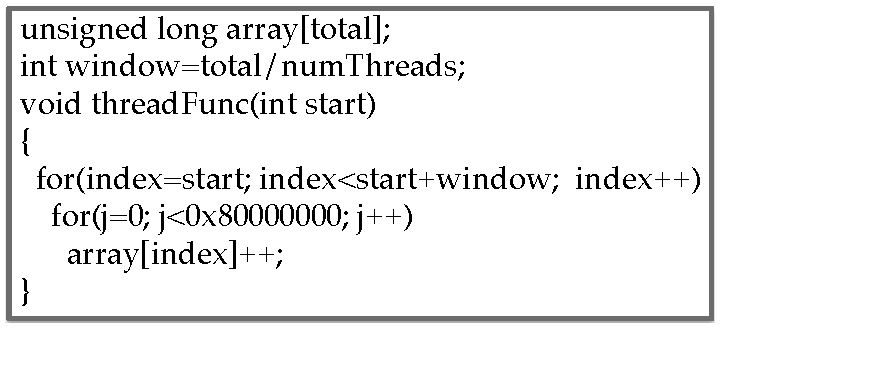
\includegraphics[width=3.1in]{figure/fscode}

}%
\hspace{20pt}
\subfigure[Performance Degradation]{%
   \label{fig:penaltyfig}
   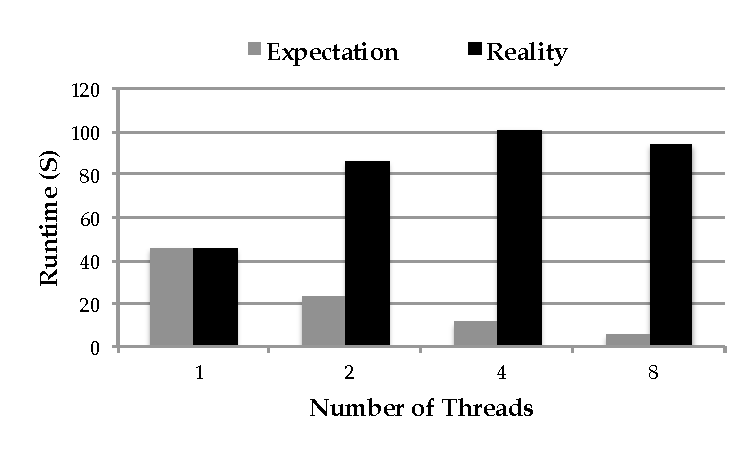
\includegraphics[width=3.1in]{figure/penalty}
}
\caption{
A false sharing example inside a multithreaded program (a) causes $13\times$ performance degradation (b) on a 8-core machine.
\label{fig:penalty}}
\end{figure*}

% Now we will talk about existing tools. 
Unlike true sharing, false sharing is generally avoidable. When threads unnecessarily share the same cache line, we can pad the data so that each thread can be forced to access a different cache line. Although the solution of fixing false sharing is somehow straightforward, detecting them is difficult and even impossible with manual checking, especially for a program with thousands or millions lines of code. Thus, it is very important to employ tools to pinpoint false sharing and provide insightful optimization guidance.

However, existing generic tools can not provide enough details about false sharing~\cite{gprof, ibs-sc, Intel:VTune}. Existing false sharing detection tools fall short in several ways. First, most tools can not distinguish true and false sharing, requiring unnecessary manual efforts to identify optimization opportunities~\cite{falseshare:binaryinstrumentation1,detect:ptu,detect:intel,falseshare:binaryinstrumentation2,DProf, qinzhao, OSdetection, mldetect, Wicaksono11detectingfalse, openmp}. Second, software-only tools~\cite{falseshare:binaryinstrumentation1,falseshare:binaryinstrumentation2,falseshare:simulator, Predator} introduce very high runtime overhead, preventing them from uses in deployment environment. Third, OS-related tools have limitations, either with custom OS support~\cite{OSdetection}, or work with special applications~\cite{Sheriff}. Fourth, to the best of our knowledge, no prior tool assesses the benefit from eliminating the false sharing. Without this information, many optimization efforts may lead to only trivial or no performance improvement.

\vspace{0.2in}

%\subsection*{Contributions}

This paper, \cheetah{}, is going to address these issues and has the following contributions:

\begin{itemize} 

% The first one is overrated. We can't do that. 
\item {\bf First Approach to Predict False Sharing Impact.} This paper introduces the first approach to predict the performance impact of fixing false sharing instances inside multithreaded programs. Based on our evaluation, \cheetah{} can precisely predict the performance improvement, with less than 10\% difference. By ruling out trivial instances, we can avoid unnecessary manual effort as much as possible. 

\item {\bf An Efficient and Effective False Sharing Detection Tool.} This paper presents \cheetah{}, an efficient false sharing detector with only 7\% performance overhead, by utilizing the Performance Monitoring Units (PMU) that are available on modern hardware. \cheetah{} can report precise information of false sharing problems, by pointing out the lines of code or the name of variables with problems. \cheetah{} is very convenient to use, which is a library that can be preloaded (using \texttt{LD\_PRELOAD} or can be linked to: there is no need to change or recompile the programs, or to modify the underlying operating system.
%which does not need custom OS,  or recompilation and changing of programs. 

\end{itemize}

The remainder of this paper is organized as follows. 
%Section~\ref{sec:overview} introduces the background of false sharing and the motivation of a new detection tool. 
Section~\ref{sec:detect} describes the design and implementation of false sharing detection tool. Section~\ref{sec:predictimprove} introduces the assessment of performance impact of false sharing. Section~\ref{sec:eval} presents experimental results, including effectiveness, performance overhead, and the precision of assessment. Section~\ref{sec:discuss} addresses main concerns on hardware dependence, performance and effectiveness. Section~\ref{sec:relatedwork} discusses related work and Section~\ref{sec:conclusion} concludes this paper. 



